\documentclass[a4paper, 11pt, final, garamond]{book}
\usepackage{cours-preambule}

\raggedbottom

\makeatletter
\renewcommand{\@chapapp}{Travaux pratiques -- TP}
\makeatother

\let\SavedIndent\indent
\protected\def\indent{%
  \begingroup
    \parindent=\the\parindent
    \SavedIndent
  \endgroup
}
\setlength{\parindent}{0pt}

\begin{document}
\setcounter{chapter}{10}

\chapter{Cin\'etique d'une r\'eaction de saponification par conductim\'etrie}
\section{Objectifs}

\begin{itemize}
    \item Utiliser une méthode conductimétrique pour vérifier un ordre global et
        pour déterminer la valeur d'une constante de vitesse $k$.
    \item Se placer dans des conditions expérimentales de proportions
        stœchiométriques.
    \item Déterminer une énergie d'activation. 
\end{itemize}

\section{S'approprier}
\subsection{Introduction}

La réaction de saponification est l'hydrolyse basique (en présence d'ions
$\ce{OH^-}$) des esters, cette réaction permet la synthèse des savons. Le savon,
produit domestique utilisé depuis des milliers d'années est à l'origine un
mélange de graisse animale fondue et de cendres. En 1823, Eugène
\textsc{Chevreul}, chimiste français, découvre que les triesters présents dans
les corps gras, réagissent avec la soude (base qui était jadis apportée par les
cendres) pour former le savon.

\subsection{Le principe de la conductimétrie}

Cette méthode repose sur l'existence d'ions en solution et sur leur capacité à
faciliter le passage d'un courant. La nature des ions et leurs concentrations
modifient la conductance $G$ du système (grandeur qui est l'inverse de la
résistance $R$) exprimée en \si{S} (Siemens). Plus le milieu est propice au
passage du courant, plus la conductance est élevée. Celle-ci est reliée à trois
paramètres principaux~:

\begin{enumerate}
    \item la conductivité $\sigma$ du système
    \item la longueur $\ell$
    \item la section $S$ de la cellule
\end{enumerate}

La conductance s'exprime alors selon
\[G = \frac{\sigma S}{\ell}\]

Ainsi, on ne parle pas de conductance \cancel{de la solution}, puisque la
conductance dépend de la cellule de mesure et de sa géométrie. L'unité de
conductivité est le $\si{S.m^{-1}}$~; le quotient $K = \ell / S$ est appelé
constante de cellule. Ainsi, on a $G = \sigma / K$. La mesure de la conductance
s'effectue avec un conductimètre, qui est en fait un ohmmètre.\bigbreak

La conductivité $\sigma$ de la solution peut alors s'exprimer par la \textbf{loi
de Kohlrausch}, exprimée sous une forme avec la chage de l'ion~:
\begin{rprop}{Loi de \textsc{Kohlrausch}}
    \[\boxed{\sigma = \sum_{i} \lambda_i \left|z_i\right| [{\rm X}_i]}\]

    Avec~:
    \begin{itemize}
        \item $\lambda_i$ la conductivité molaire ionique de l'ion ${\rm X}_i$ (en
            $\si{S.m^2.mol^{-1}}$) donnée dans les tables
        \item $z_i$ la charge de l'ion ${\rm X}_i$
        \item $[{\rm X}_i]$ la concentration de l'ion ${\rm X}_i$
    \end{itemize}
\end{rprop}

\begin{rror}{Important}
    \begin{center}
        \bfseries
        La conductivité $\sigma$ de la solution prend en compte tous les ions
        présents dans la solution. Il faut donc faire l'inventaire des ions en
        solution avec soin.
    \end{center}
\end{rror}

En supposant que l'on ne fait varier que d'une unique espèce ionique (et donc
conductrice) dans la solution, on pourra noter $c = [{\rm X}_i]$ la
concentration de cette espèce. La \textbf{courbe d'étalonnage} est alors la
représentation graphique de $\sigma = f(c)$ obtenue avec l'ensemble des points
de coordonnées $(c_i~; \sigma_i)$ où $\sigma_i$ sont les conductivités des
différentes solutions étalons $S_i$ de concentration $c_i$. Connaissant la
conductivité $\sigma_0$ de la solution $S_0$ inconnue, on en déduit grâce à la
courbe d'étalonnage la concentration molaire $c_0$ de la solution $S_0$.

\section{Analyser}
\subsection{Données numériques utiles}

\begin{rdefi}{Données}
    \begin{minipage}{0.50\linewidth}
        \centering
        \begin{tabular}{lccc}
            \toprule 
            Ions &
            \ce{HO-} &
            \ce{CH3CO2-} &
            \ce{Na+}\\
            $\lambda$ \newline
            (\si{mS.m^2.mol^{-1}}) &
            \num{19.86} &
            \num{4.09} &
            \num{5.01}\\
            \bottomrule
        \end{tabular}
    \end{minipage}
    \begin{minipage}{0.50\linewidth}
        \centering
        \begin{tabular}{lcccc}
            \toprule 
            Élément & Na & C & O & H\\
            Masse molaire (\si{g.mol^{-1}}) &
            23 &
            12 & 
            16 &
            1\\
            \bottomrule
        \end{tabular}
    \end{minipage}
    \begin{itemize}
        \item Densité de l'éthanoate d'éthyle pur~: $d = \num{0.90}$~;
        \item Constante des gaz parfaits~: $R = \SI{8.314}{J.K^{-1}.mol^{-1}}$
    \end{itemize}
\end{rdefi}

\subsection{Préliminaires}

La réaction étudiée ici est la saponification de l'éthanoate d'éthyle par la soude à température ambiante. C'est une réaction \textbf{totale et lente}.

      \begin{center}
        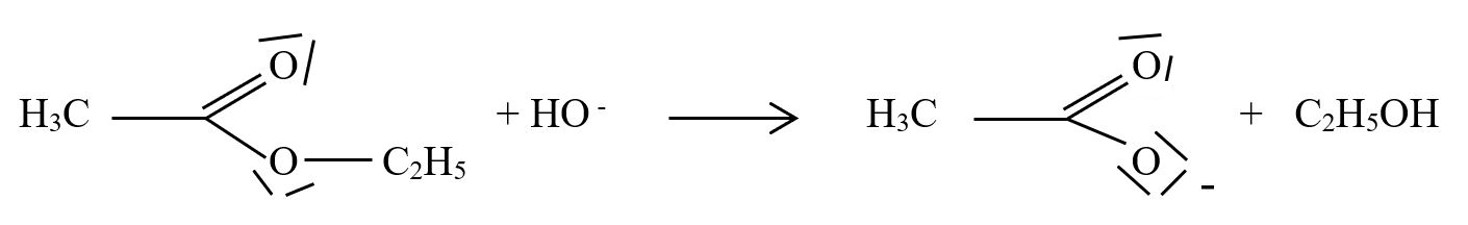
\includegraphics[width=0.7\textwidth]{reaction}
      \end{center} 
      
Par souci de simplicité, on notera par la suite la réaction~: \hfill
\fbox{$\ce{RCOOR}'+\ce{OH^-} \rightarrow \ce{RCOO^-} + \ce{R}'\ce{OH}$}

\vspace{-10pt}
\subsubsection{Rappels de chimie organique}

\vspace{-10pt}
\begin{rexem}{\tiny Questions}
    \begin{enumerate}[label*=\sqenumi]
        \item Quelle est la classe fonctionnelle (ou famille) de l'éthanoate
            d'éthyle~? Quelle est son groupe caractéristique~? Quelle est sa formule
            semi-développée~? Nommer les deux produits obtenus.
    \end{enumerate}
\end{rexem}

\vspace{-10pt}
\subsubsection{Choix de la méthode d'étude}

\vspace{-10pt}
\begin{rexem}{\tiny Questions}
    \begin{enumerate}[label*=\sqenumi, start=2]
        \item Justifier que la conductimétrie soit une méthode particulièrement
            adaptée pour le suivi cinétique de cette réaction.
    \end{enumerate}
\end{rexem}

\vspace{-10pt}
\subsubsection{Sécurité}

\vspace{-10pt}
\begin{rexem}{Questions}
    \begin{minipage}{0.55\linewidth}
        \begin{enumerate}[label=\sqenumi, start=3]
            \item On peut voir ces pictogrammes sur les étiquettes des flacons~: que
                signifient-t-ils~? quelles précautions faut-il prendre~?
        \end{enumerate}
        Vous pourrez consulter\\
        \url{http://www.inrs.fr/media.html?refINRS=ED%204406}
    \end{minipage}
    \hfill
    \begin{minipage}{0.40\linewidth}
        \begin{center}
            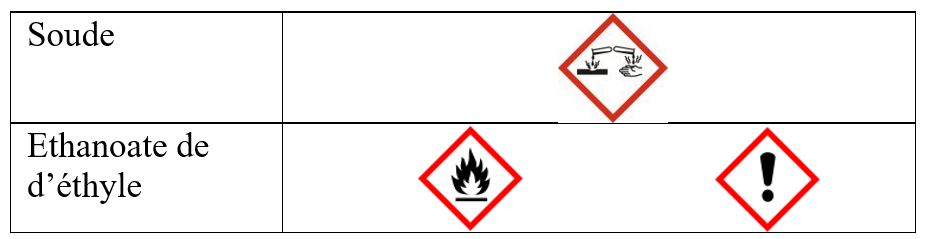
\includegraphics[width=\linewidth]{picto}
        \end{center} 
    \end{minipage}
\end{rexem}

\subsection{\'Etude théorique de la cinétique}

On cherche à vérifier que cette réaction est d'ordre global 2 avec un ordre
partiel de 1 par rapport à chacun des réactifs.

\begin{rexem}{Questions}
    \begin{enumerate}[label=\sqenumi, start=4]
        \item Ecrire la loi de vitesse correspondante.
        \item Les conditions expérimentales sont choisies pour que l'on soit dans
            les proportions stœchiométriques. De plus à l'instant initial, il n'y a
            pas encore de produits. Ainsi, 
            \[[\ce{RCOOR}']_0 = [\ce{OH-}]_0 = c_0 \qet [\ce{RCOO-}]_0 = 
            [\ce{R}'\ce{OH}]_0 = 0\]
            Simplifier, dans ces conditions, la loi de vitesse précédente.
        \item Faire un tableau d'avancement sur les concentrations aux instants $t =
            0$, $t$ quelconque, et $t\to \infty$ (noté $t_\infty$) sachant que la
            réaction est supposée \textbf{totale}. On introduira pour plus de
            commodité d'écriture $x$ l'avancement volumique $x = \xi / V$.
        \item Déterminer une équation différentielle vérifiée par $x$. Puis intégrer
            cette équation à l'aide de la méthode de séparation des variables pour
            obtenir $x$ en fonction de $t$ explicitement. Quel graphe faudrait-il
            tracer, connaissant $x(t)$, pour vérifier que la réaction est bien
            d'ordre 2~?
        \item Exprimer en fonction des concentrations des différentes espèces X$_i$
            et de leurs conductivités molaires ioniques $\lambda_i$, la
            conductivité $\sigma_0$ de la solution à l'instant initial, celle
            $\sigma_\infty$ à un temps infini, et enfin $\sigma$ à l'instant $t$.
        \item \leftcenters{Montrer qu'alors}
            {$\dfrac{\sigma_0-\sigma_\infty}{\sigma-\sigma_\infty} =
            \dfrac{c_0}{c_0-x}$}
        \item En déduire que si la vitesse est bien telle qu'elle a été supposée
            (c'est-à-dire suivant une loi d'ordre global 2), la relation suivante
            doit être vérifiée~: 
            \[\dfrac{\sigma_0-\sigma_\infty}{\sigma-\sigma_\infty} = c_0 k t +1\]
        \item Sachant que l'on va mesurer les conductivités, quel graphe doit-on
            tracer pour obtenir une droite si l'ordre de la réaction est bien de 2~?
            Comment pourra-t-on en déduire la constante de vitesse de la réaction~?
    \end{enumerate}
\end{rexem}

\section{Réaliser}

\begin{NCror}[width=\linewidth]{Important}
    \begin{center}
        \bfseries
        Le port de la blouse fermée et des lunettes est obligatoire durant
        l'ensemble du TP. Les cheveux longs doivent être attachés.
    \end{center}
\end{NCror}

\subsection{Protocole expérimental}

\subsubsection{Solutions disponibles}
\begin{itemize}
    \item \leftcentersright{Solution de soude}{($\ce{Na^+} +
        \ce{OH^-}$)}{$\SI{0,100}{mol.L^{-1}}$}~;
        \vspace{-15pt}
    \item \leftcentersright{Solution d'éthanoate (ou acétate)
        d'éthyle}{($\ce{RCOOR}'$)}{$\SI{0,100}{mol.L^{-1}}$}~;
        \vspace{-15pt}
    \item \leftcentersright{Solution d'acétate de sodium}{($\ce{RCOO^-} +
        \ce{Na^+}$)}{$\SI{5.0e-2}{mol.L^{-1}}$}.
\end{itemize}

\subsubsection{Matériel disponible}
\begin{itemize}
    \item Verrerie usuelle~:\smallbreak
        \begin{minipage}{0.50\linewidth}
            \begin{itemize}
                \item bécher ($\SI{100}{mL}$, $\SI{150}{mL}$, $\SI{250}{mL}$)
                \item fioles jaugées ($\SI{50,0}{mL}$, $\SI{100,0}{mL}$)
            \end{itemize}
        \end{minipage}
        \begin{minipage}{0.50\linewidth}
            \begin{itemize}
                \item pipettes jaugées ($\SI{10,0}{mL}$, $\SI{20,0}{mL}$)
                \item éprouvettes graduées ($\SI{10}{mL}$, $\SI{50}{mL}$)
            \end{itemize}
        \end{minipage}
    \item Conductimètre.
    \item Agitateur magnétique.
    \item Thermomètre, chronomètre, ordinateur avec regressi.
\end{itemize}

\vspace{-10pt}
\begin{rexem}{\tiny Question}
    \begin{enumerate}[label=\sqenumi, start=12]
        \item \textbf{Discuter de la nécessité d'étalonner le conductimètre}.
    \end{enumerate}
\end{rexem}
\vspace{-10pt}

\subsubsection{Détermination de $\sigma_0$ et de $\sigma_\infty$}
\begin{rexem}{Questions}
    \vspace{-10pt}
    \begin{enumerate}[label=\sqenumi, start=13]
        \item $\sigma_0$ ne peut pas être déterminée précisément à partir du mélange
            réactionnel pris à $t = 0$. \textbf{Pourquoi}~?
        \item Afin de déterminer précisément $\sigma_0$, réaliser une solution
            équivalente au milieu réactionnel initial mais dont la conductivité
            n'évolue pas. \textbf{Expliquer votre démarche et votre protocole
            expérimental}.
        \item $\sigma_\infty$ est également difficile à déterminer précisément à
            partir du mélange réactionnel. \textbf{Pourquoi}~?
        \item Afin de déterminer précisément $\sigma_\infty$, réaliser une solution
            équivalente au milieu réactionnel final mais dont la conductivité
            n'évolue pas. \textbf{Expliquer votre démarche et votre protocole
            expérimental}.
    \end{enumerate}
\end{rexem}
\vspace{-10pt}

\subsubsection{Suivi conductimétrique à température ambiante}

\begin{enumerate}
    \item Prélever $\SI{50}{mL}$ de soude mesurés avec une fiole jaugée et
        mettre en place le dispositif d'agitation et le  régler pour que la
        vitesse soit faible et ne touche pas à l'électrode.
\end{enumerate}
\vspace{-10pt}
\begin{brapp}{Rappel}
    \centering
    Il est préférable de faire des mesures de conductimétrie sans
    agitation. Mais ici ce n'est pas possible car il faut que les
    concentrations soient uniformes en solution. Pour que la
    perturbation soit moindre, il ne faut pas changer la vitesse
    d'agitation au cours de la réaction.
\end{brapp}
\vspace{-10pt}
\begin{enumerate}[resume]
    \item Ajouter alors le volume adéquat d'éthanoate d'éthyle mesuré avec une
        fiole jaugée pour que les solutions soient introduites dans les
        proportions stœchiométriques et mettre en route le chronomètre.
    \item Toutes les 30 secondes, relever la conductivité de la solution au
        cours du temps et ce pendant 20 min environ.
    \item Faire un schéma du dispositif expérimental.
\end{enumerate}

\section{Valider}
\subsection{Exploitation des mesures}

\begin{enumerate}[label=\sqenumi, start=17]
    \item Recopier votre tableau de valeur dans latispro ou régressi.
    \item Expliquer l'allure décroissante de la courbe $\sigma = f(t)$.
    \item Tracer le graphe nécessaire à la vérification de l'ordre 2. L'imprimer
        ainsi que sa modélisation. 
    \item Conclure quant à l'ordre global de la vitesse de la réaction étudiée.
    \item En déduire la valeur de la constante de vitesse à la température
        ambiante en précisant son unité.
\end{enumerate}

\subsection{Influence de la température~; détermination de l'énergie d'activation}

Les mêmes expériences ont été réalisées à des températures différentes grâce
à des bains thermostatés. Les valeurs des constantes de vitesse selon la
température ont été rapportées dans le tableau suivant, où l'unité de la
constante de vitesse $k$ est celle trouvée dans la partie précédente
(exploitation des mesures) avec le temps en secondes.

\begin{center}
    \begin{tabular}{ccccc}
        \toprule 
        $\theta$ (\si{\degreeCelsius}) &
        Ambiante & 35 & 40 & 45 \\
        $k$ (\si{SI}) &
        Votre valeur~! & \num{0.188} & \num{0.257} & \num{0.356}\\
        \bottomrule
    \end{tabular}
\end{center}

\begin{enumerate}[label=\sqenumi, start= 22]
    \item Rappeler la loi d'Arrhénius~; 
    \item Faire la régression linéaire (sur régressi ou sur votre calculatrice)
        nécessaire à la détermination de l'énergie d'activation de cette
        réaction~; Préciser son unité. 
\end{enumerate}

% \vspace{3cm}
% 
% \begin{programme}{}
% 
% \vspace{1cm}
% \begin{itemize}
% \item ƒtablir une loi de vitesse à partir du suivi 
% temporel d'une grandeur physique. 
% \item Suivi cinétique de transformations chimiques 
% \item Suivi en continu d'une grandeur physique. 
% \item Mettre en œuvre une méthode de suivi temporel. 
% \item Exploiter les résultats d'un suivi temporel de 
% concentration pour déterminer les caractéristiques 
% cinétiques d'une réaction. 
% \item Proposer et mettre en œuvre des conditions 
% expérimentales permettant la simplification de la loi 
% de vitesse. 
% \item Déterminer la valeur d'une énergie d'activation. 
% \item Pratiquer une démarche expérimentale pour 
% déterminer une concentration ou une quantité de 
% matière par spectrophotométrie UV-Visible.
% \end{itemize}
% \end{programme}

\end{document}

